\section{Problem Formulation}
\label{sec:problem-formulation}

\Cref{fig:system-model} shows the system model that has three different entities.
\begin{enumerate*}[label=(\roman*)]
\item \emph{Key center}.
A trusted entity that is involved only in the initialization of the system to generate the keys for the other actors in the system.
\item \emph{Users}.
Train their local models, share their trained gradients with the servers, and get the aggregated gradient from the servers to update the model weights for a specific iteration $t$.
\item \emph{Servers}.
The system comprises two servers namely, $S_1, S_2$.
The two servers communicate together to defend against model poisoning attacks. and to calculate the aggregated gradient.
\end{enumerate*}

\begin{figure}[htb]
\centering
  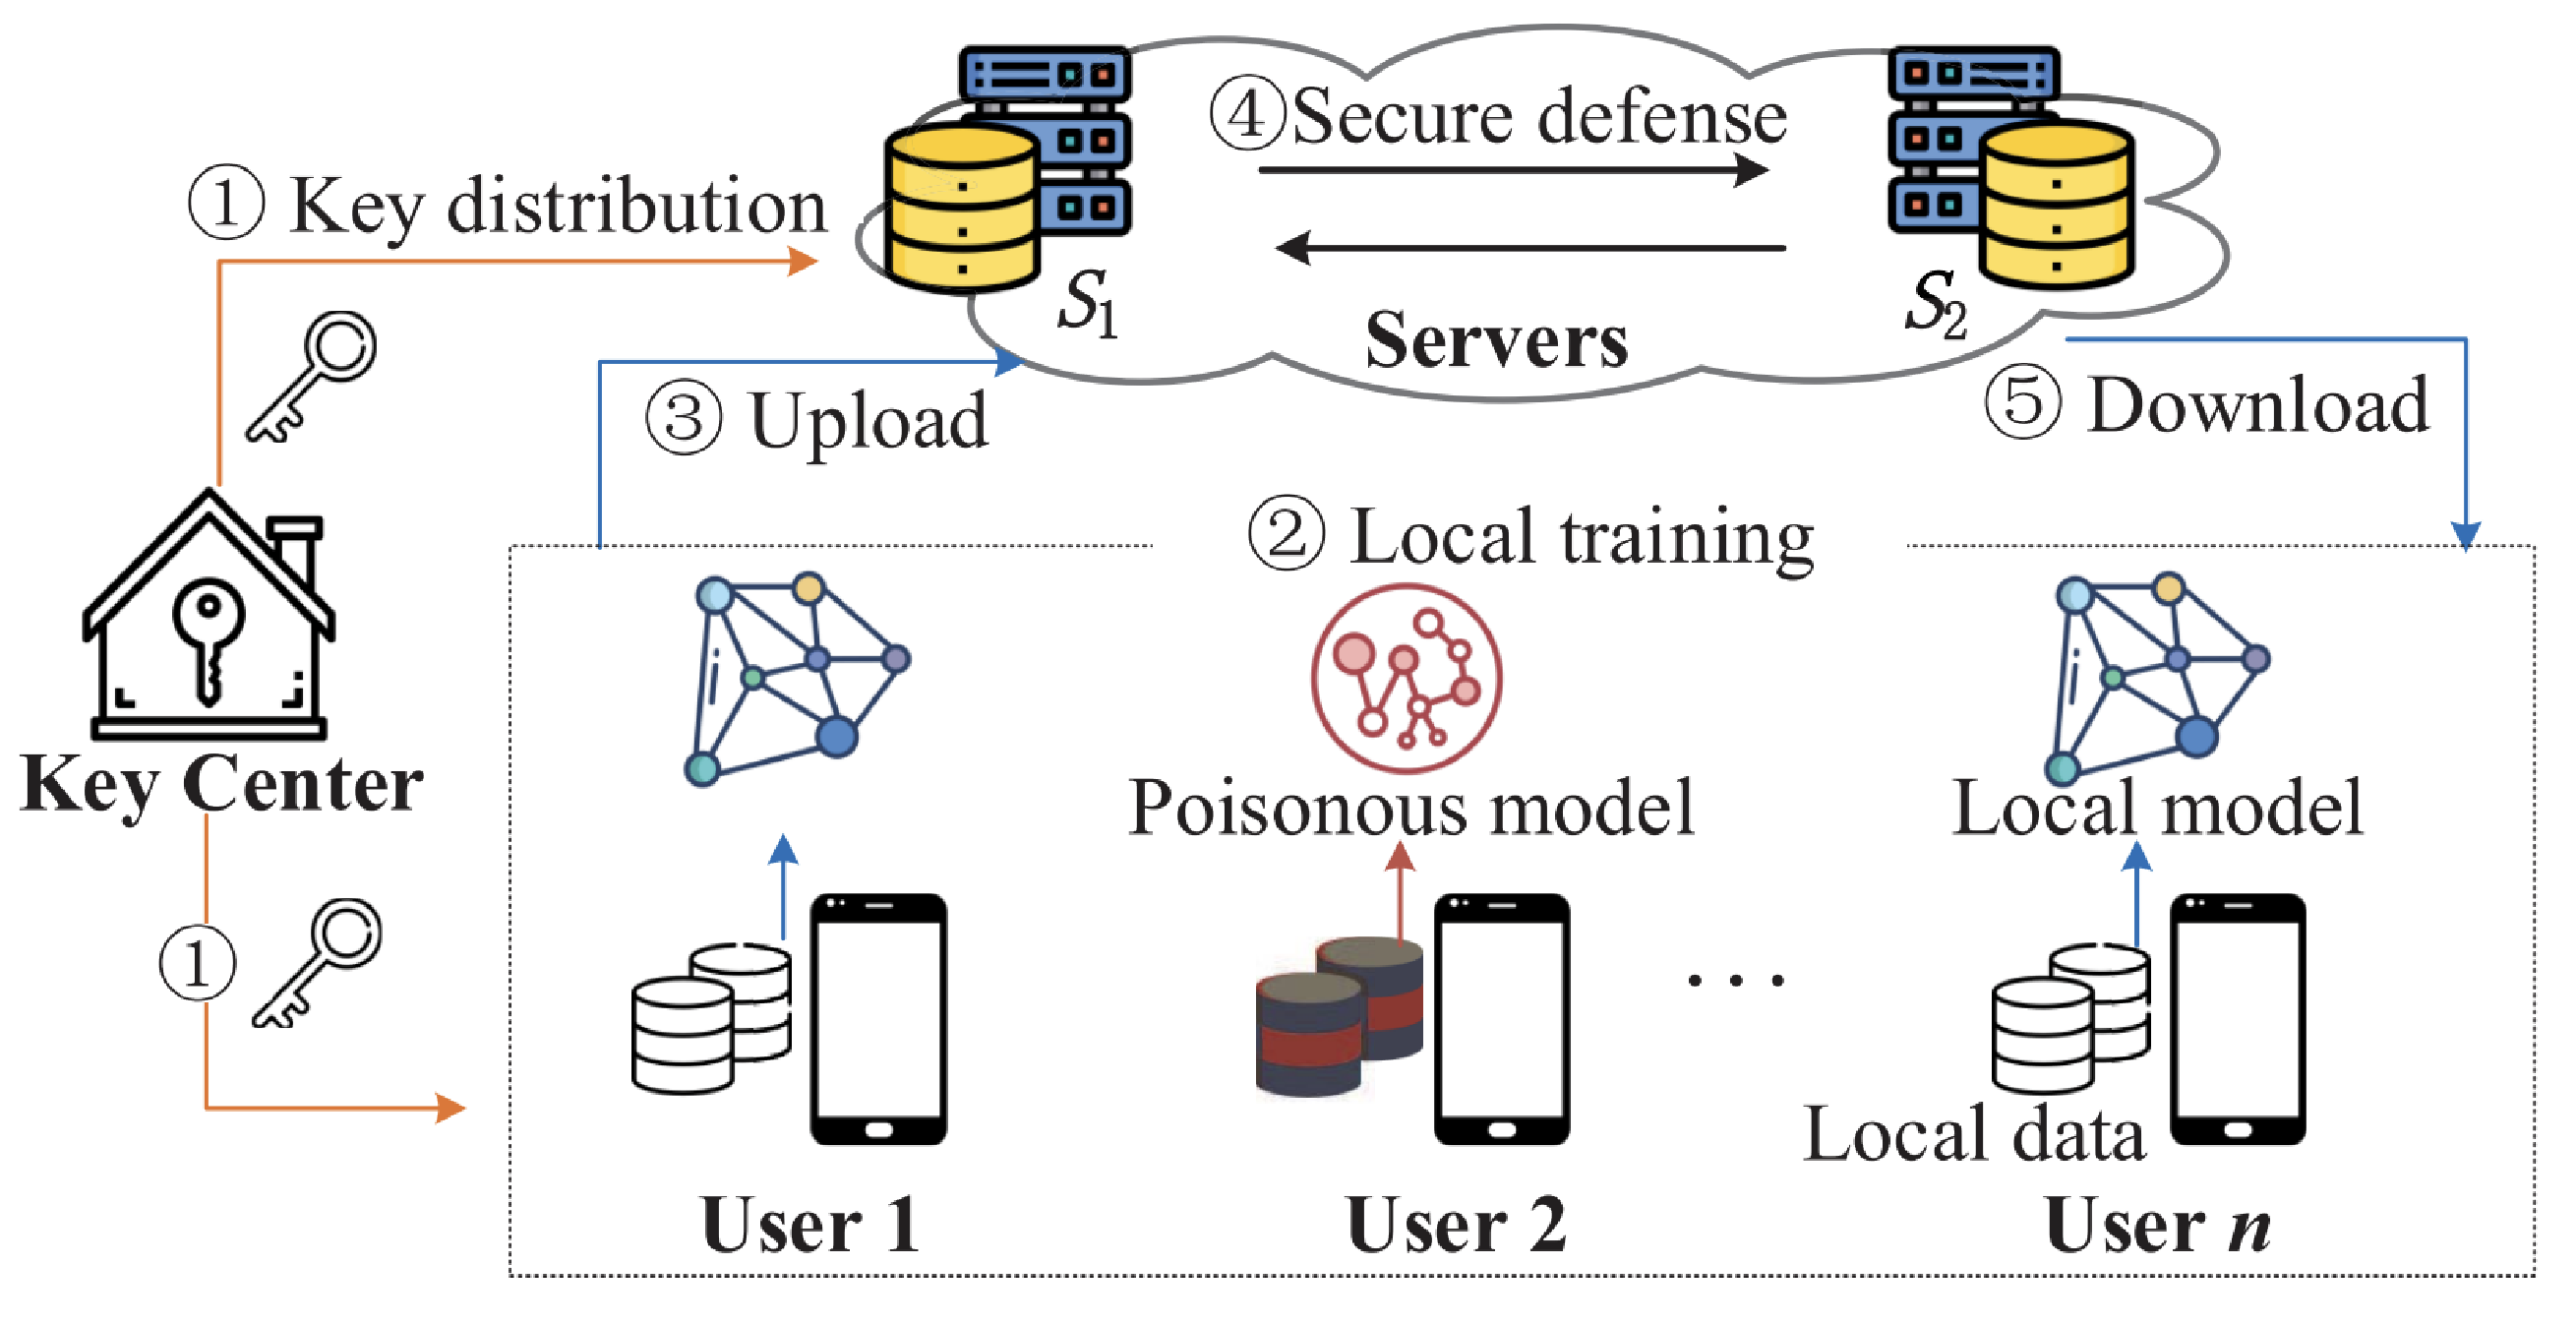
\includegraphics[width=0.8\linewidth]{resources/system-model.pdf}
  \caption{System Model}
  \label{fig:system-model}
  %\vspace{-5mm}
\end{figure}

For the threat model, the two servers are assumed to be non-colluding honest-but curious entities, similar to the model used in \cite{mohassel2017secureml}.
The users can act maliciously by submitting poisonous gradients $[[g_i^*]]$
The model poisoning attack is defined in \cite{fang2020local} and can be described as follows:
\begin{enumerate*}
    \item Adversary corrupts the local training process to decrease the accuracy of the federated model.
    \item Adversary controls one or more malicious users $U^*$.
    \item Adversary tries to fool poison the gradients by understanding the crafting the malicious gradients.
\end{enumerate*}

% TODO: AB: I may need to add the design goals based on the size.
